\section{Hybrid Attitude Controller}

Dynamic discontinuous hybrid controller, global asymptotic stability, local exponential stability, state feedback for $\omega$ and $q$. Capable of detumbling. \cite{globalAttController}

One way of describing rotation in 3D Eucledian space is by using Euler sequences consisting of 3 rotational values. Euler rotation sequences can use combinations of roll, pitch and yaw. There's an inherent problem with Euler rotation, that makes controlling them an issue, i.e. they are disposed to singularities. Certain orientations might described by an infinite amount of different sequences. This situation can arise when the rotations are made in such a way that rotation axes align with each other. This issue is called the gimbal lock. The result is that given a attitude demand, the corresponding Euler rotations can not be unambiguously deducted, unless extra constraints are used.

Quaternion based rotation representation significantly improves control capabilities. Quaternions are not susceptible to singularities. The only problem with quaternion representation is the so-called double coverage, i.e. rotation by $-\vec{q}$ represents the same rotation as rotation by $-\vec{q}$. This becomes obvious from the rotation equation \ref{eq:doubleCover}.

\begin{equation}
\label{eq:doubleCover}
\vec{q} \vec{v} \vec{q}^{-1} = 	(\vec{-q}) \vec{v} (\vec{-q}^{-1})
\end{equation} 

The attitude control goal can be described as keeping the orientation demand $\vec{q}$. According to  \cite{globalAttController}, it is impossible to design a globally stabilizing quaternion based state feedback that is robust to measurement noise. The quaternion-based robust hysteric feedback controller which is capable of globally asymptotically stabilizing a rigid body is described subsequently. It can be considered as a more robust extension of classical state feedback controller.


The dynamics of a rigid body is described in equation \ref{eq:dynSimple}. For clarity of the control method, disturbance torques are emitted from the equation. For more details, refer to Appendix ... .

\begin{equation}
\label{eq:dynSimple}
\underline{I}_s \vec{\dot{\omega}} = \underline{\omega}^\times \underline{I}_s \vec{\omega} + \vec{N_{ctrl}}
\end{equation}

The control goal can be clearly described with rotation matrices. Rotation matrices use 9 variables to describe a rotation, but they have the advantage of being non-ambiguous. The rotation error can be described using equation \ref{eq:rotationError}. 

\begin{equation}
\label{eq:rotationError}
\underline{R}_e = \underline{R}(\vec{q_d})^T \underline{R}(\vec{q})
\end{equation}

The goal is to align the $\underline{R}(\vec{q})$ with $\underline{R}(\vec{q_d})$. If that demand is satisfied, $\underline{R}_e$ becomes $\underline{I}$ identity matrix. In quaternion representation, this goal corresponds to having having a unit quaternion with the scalar element being $\pm 1$, according to equation \ref{eq:stabilityQuat}. 

\begin{equation}
\label{eq:stabilityQuat}
\underline{R}_e = \underline{I} \xrightarrow{equivalent} \vec{q_e}  = \pm	\begin{bmatrix}
0 \\
0 \\
0 \\
1
\end{bmatrix} 	
\end{equation}

Because of the double coverage property of quaternions, stabilizing an attitude, stabilization has to be done on a two equilibrium points corresponding to $\vec{q_e}$ in equation \ref{eq:stabilityQuat}. According to \cite{globalAttController}, robust and global stabilization on this set is impossible to achieve using non-hybrid discontinuous state feedback in the presence of sensor noise. The paper proposes a hybrid, discontinuous, robust, gloablly asymptotically stabilizing attitude control method instead. A hybrid system is a system in which state changes can vary between being continuous or discrete.

The state changes are controlled by the following rules. Controller state storing information about which of the double covering quaternions should be tracked is introduced as $x_c \epsilon  \left\lbrace -1,1 \right\rbrace $. The rule for choosing between discrete or continuous control mode is presented in equation \ref{eq:contDiscont}.

\begin{align}
\label{eq:contDiscont}
C:= \left\lbrace (\vec{q},\vec{\omega},x_c) \in \mathbb{S}^3 \times \mathbb{R}^3 \times \left\lbrace -1,1 \right\rbrace : x_c q_4 \geq -\delta \right\rbrace  \\
\nonumber D:= \left\lbrace (\vec{q},\vec{\omega},x_c) \in \mathbb{S}^3 \times \mathbb{R}^3 \times \left\lbrace -1,1 \right\rbrace : x_cq_4 \leq -\delta \right\rbrace 
\end{align}

where $\delta \in (0,1)$ is the threshold parameter. If $(\vec{q},\vec{\omega},x_c) \in C$, i.e. the controller is running in continuous mode, the governing equations are according to equation \ref{eq:globalCont}. When $(\vec{q},\vec{\omega},x_c) \in D$, $x_c$ swaps sign instantaneously. Because of the $\delta$ thresholding, two swaps don't happen in infinitesimally small time.  

\begin{align}
	\label{eq:globalCont}
\dot{x}_c = 0, & (\vec{q},\vec{\omega},x_c)  \in C \\
\label{eq:globalDiscont}
x_c^+ = -x_c, & (\vec{q},\vec{\omega},x_c) \in D\
\end{align}

Equation \ref{eq:globalControlInput} describes the generated negative feedback control signal. $K_q$ is the adjustable orientation error gain, $K_e$ is an also adjustable parameter for angular velocity gain.

\begin{equation}
\label{eq:globalControlInput}
\vec{u} = -K_q x_c \vec{q}_{e, 1:3} -K_\omega \vec{\omega_e}
\end{equation}
\todo{how does it handle nonzero omega demand?}

%\begin{align}
%	\label{eq:contDiscont}
%	x_c q_4 \geq -\delta \xrightarrow{}  Continuous \\
%	\nonumber x_c q_4 < -\delta \xrightarrow{}  Discontinuous
%\end{align}

\todo{add to nomenclature}


%\[
%\begin{array}{l}
%%\dot{x}_c = 0, (\vec{q},\vec{\omega},x_c) \in C\ \\ 
%x_c^+ = -x_c, (\vec{q},\vec{\omega},x_c) \in D\ \\ 
%%\vec{u} = -c x_c \epsilon -K_\omega \vec{\omega} \\
%%C:= \left\lbrace (\vec{q},\vec{\omega},x_c) \in \mathbb{S}^3 \times \mathbb{R}^3 \times \left\lbrace -1,1 \right\rbrace : x_c\eta \geq -\delta \right\rbrace  \\
%%
%%D:= \left\lbrace (\vec{q},\vec{\omega},x_c) \in \mathbb{S}^3 \times \mathbb{R}^3 \times \left\lbrace -1,1 \right\rbrace : x_c\eta \leq -\delta \right\rbrace 
%\end{array}
%\]

\subsubsection{Detumbling}

After a satellite is ejected from its rocket, it might be rotating quite fast. The first task of the satellite attitude controller is detumbling the satellite, preparing for normal operation. The hybrid attitude controller is capable of doing that. This means that the hybrid attitude controller is a good nominee for being the attitude controller for every operation mode. A simulation was made where the satellite's initial angular velocity is unrealistically high, the goal being to stabilize the satellite to point at the nadir. The controller saturates at $\pm 2 \dot 10^{-3} Nm$, characteristic of the reaction wheels. At the current level of analysis, motor and magnetorquer models are omitted, it is assumed that the actuators satisfy the attitude controller's torque demand. Simulation results with actuator models are presented in subsequent chapters.
\todo{Simulate desat with motor and mt model} 
\todo{set Kq to zero for detumbling}

\begin{figure}[H]
	\centering
	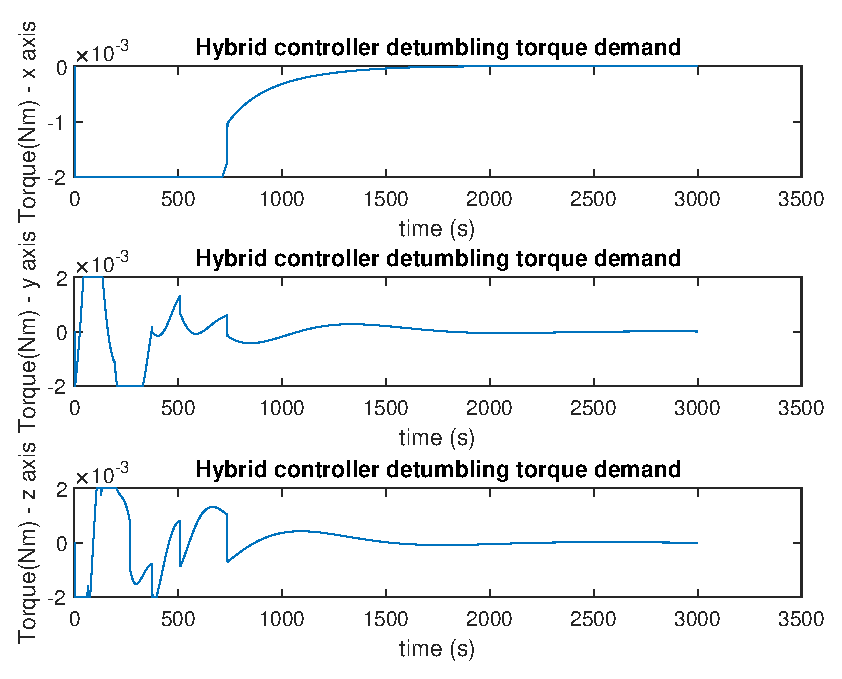
\includegraphics[width=0.7\linewidth]{figures/detumbling}
	\caption{Hybrid controller detumbling torque demand}
	\label{fig:detumbling}
\end{figure}

\begin{figure}[H]
	\centering
	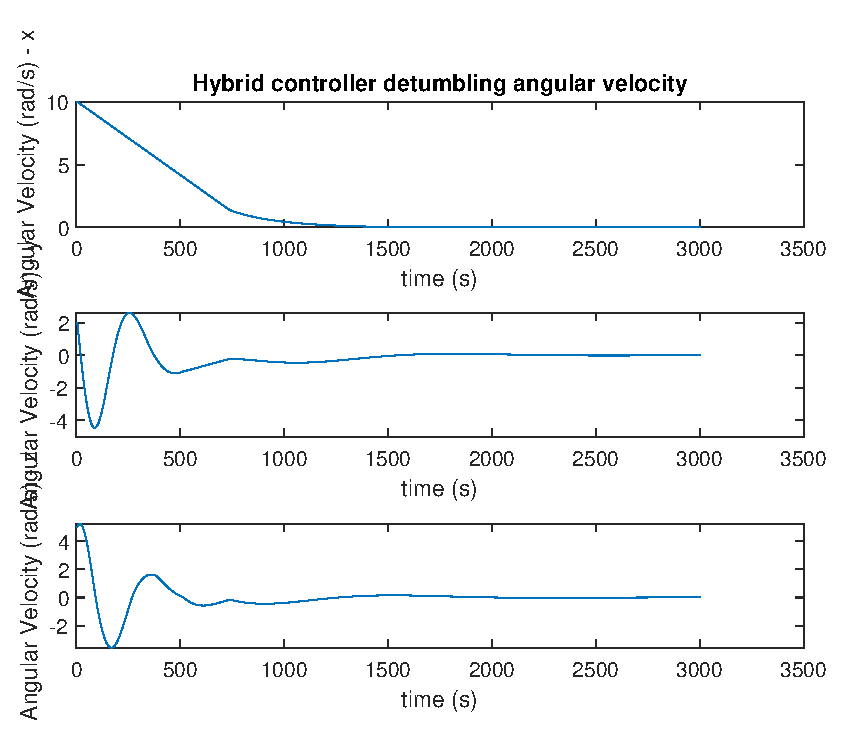
\includegraphics[width=0.7\linewidth]{figures/detumbling3}
	\caption{Hybrid controller detumbling angular velocity}
	\label{fig:omega}
\end{figure}

